The compelling physics case in Section~\ref{sec:physics} is constructed 
based on a set of solid estimates for measurements of various observables at the ILC. 
The observables related to Higgs physics are outlined in Table~\ref{tab:higgserrors} 
and~\ref{tab:WWerrors}, mostly $\sigma$ and $\sigma\cdot BR$ measurements
using the Higgs production processes shown in Fig.\ref{fig:HiggsProdILC},
 and will be explained in detail in this section. 
By solid it means that the estimates are obtained after having performed
full simulation of experimental physics analyses. 

\begin{figure}
\begin{center}
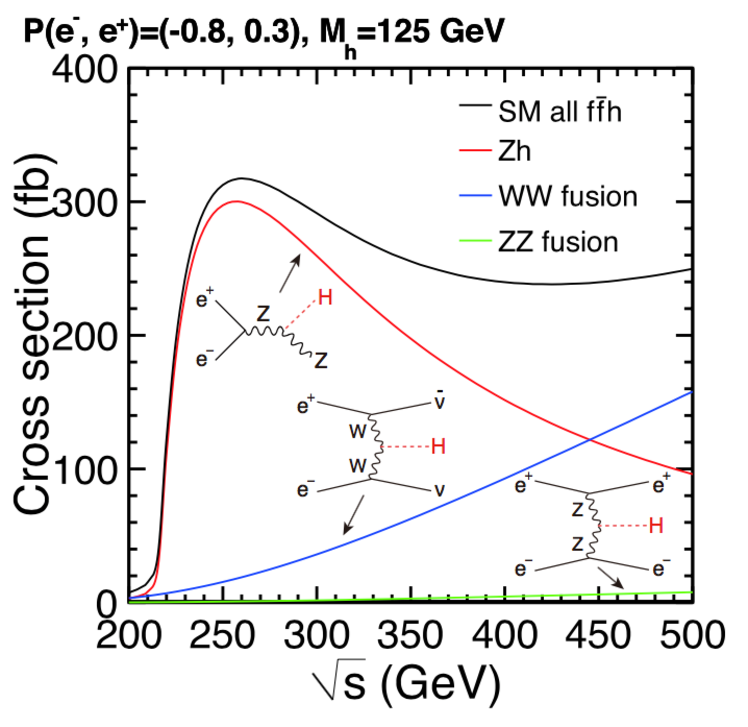
\includegraphics[width=0.85\hsize]{chapters/figures/xsec_h_ILC_left.pdf}
\end{center}
\caption{Cross sections for the three major Higgs production processes
  as a function of 
center of mass energy, 
from~\cite{Baer:2013cma}.}
\label{fig:HiggsProdILC}
\end{figure}

Section~\ref{sec:software} has introduced a few aspects of the full simulation
which can be defined as ``{\it detector simulation level}" and are absolutely essential: 
realistic interaction between each final state particle and 
and any part of the detector that the particle passes through, including new creation of
particles during the interaction; realistic algorithms for tracking,
particle flow analysis, vertex reconstruction and particle identification; 
resulting realistic performance of various detector resolutions for track momentum, jet energy,
and impact parameters, as well as of various efficiencies for tracking, flavor tagging, 
and isolated lepton finder. 

This section will introduce the other aspects of the full simulation which can be
defined as ``{\it event selection level}" and are mainly dealing with discrimination 
between signal and background events. As expected, the detailed strategies 
at the event selection level highly depend on what kind of observables we are going to
measure, and are elaborated in each of the following sub-sections. Before that, it is worth
emphasizing a few general features that are important to reach a solid estimate
and often are not well noticed or not fully captured in 
many fast simulation analyses in the literatures:
%{\color{red} JL: shouldn't the modelling of these be described in the software and MC sample chapter? We can mention them again here to rub the point in, of course, but the basic explanations ``[to be filled]'' should be in the previous chaper...}
%{JT: no, [to be filled] is not for "the basic explanations"}
\begin{itemize}
\item beamstrahlung and ISR
[to be filled]
\item overlay of beam background events
[to be filled]
\item full standard model background
[to be filled]
\item jet clustering and jet paring
[to be filled]
\item control of systematics 
[to be filled]
\end{itemize}

\begin{table}[htb]
\begin{center}
%\begin{tabular} {lcccccc}
\begin{tabular} {lcccccc}
\multicolumn{7}{l} {-80\% $e^-$, +30\% $e^+$ polarization:} \\  \hline
% & 250 GeV   &  & 350 GeV & & 500 GeV  &  \\
 & \multicolumn{2}{c}{250 GeV} & \multicolumn{2}{c}{350 GeV}  & \multicolumn{2}{c}{500 GeV} \\
 &  $Zh$ & $ \nu\bar\nu h$  & $ Zh$ & $\nu\bar\nu h$ & $Zh$ & $ \nu\bar\nu h$\\ 
\hline
$\sigma$  &    2.0     &    &1.8  &  &  4.2   &     \\  \hline
$h\to invis.$ &  0.86   &  &1.4 &   &   3.4 &     \\
\hline
$h\to b\bar b$  &   1.3 &  8.1 & 1.5  &  1.8  & 2.5  &  0.93  \\ 
$h\to c\bar c$ &  8.3 &   &11 & 19  &   18 & 8.8 \\ 
$h\to gg$ &  7.0 &  &8.4  & 7.7 & 15  &  5.8\\
$h\to WW$  &  4.6 &   &5.6$^*$ & 5.7$^*$ &  7.7   &  3.4\\
$h\to \tau\tau$  & 3.2 &   &4.0$^*$ & 16$^*$ &  6.1  &  9.8\\
$h\to ZZ$ & 18 &   & 25$^*$ & 20$^*$ & 35$^*$  & 12$^*$    \\ 
$h\to \gamma\gamma$  & 34$^*$ &   &39$^*$ &  45$^*$ &  47 &  27 \\ 
$h\to \mu\mu$ & 72 &   &87$^*$&  160$^*$ &  120 &  100 \\
\hline\hline
$a$  &  7.6   &     &2.7$^*$ &   &  4.0   &  \\
$b$ &  2.7  &    & 0.69$^*$ &    & 0.70   &   \\
$\rho(a,b)$  &  -99.17 &   & -95.6$^*$ &  & -84.8 &   \\
\end{tabular}
\caption{Projected statistical errors, in \%, for Higgs boson 
measurements. The errors are 
quoted for luminosity samples of 250~fb$^{-1}$
  for $\ee$ beams with -80\% electron polarization and +30\% positron
  polarization. 
  Except for the first and last segments of  each set, these are measurments
  of  $\sigma \cdot BR$, relative to the Standard Model
  expectation.
The top lines gives the error for the total cross section relative to
the Standard Model and  the 95\% confidence upper limit on the branching ratio for
Higgs to invisible decays.  The bottom lines in each half give the
expected errors on the $a$ and $b$ parameters and their correlation
(all in \%)  for $\ee\to Zh$ (see
\leqn{genZhform}.    All error estimates in this table are
based on full simulation, and the entries marked with a $^*$ are 
extrapolated from full simulation results. }  
\label{tab:higgserrors}
\end{center}
\end{table}

\begin{table}
\begin{center}
\begin{tabular} {lcccccc}
 & 250 GeV   &  & 350 GeV & & 500 GeV  &  \\
 &  $ W^+ W^-$  &  &  $ W^+ W^-$  &  &  $ W^+ W^-$  & \\
 \hline
$g_{1Z}$ & 0 .062$^*$&   &0.033$^*$ &  &0.025  &  \\
$\kappa_A $ & 0.096$^*$ &   & 0.049$^*$  &   & 0.034 &  \\
$\lambda_A$ &   0.077$^*$ &   &0.047$^*$  &  &0.037  &  \\
$\rho(g_{1Z},\kappa_A)$ & 63.4$^*$ &   &63.4$^*$  &  & 63.4 &  \\
$\rho(g_{1Z},\lambda_A)$ &  47.7$^*$ &   & 47.7$^*$  &  &47.7  &  \\
$\rho(\kappa_A,\lambda_A)$ & 35.4$^*$  &   & 35.4$^*$  &  & 35.4  &  
\end{tabular}
\caption{Projected statistical errors, in \%, for $\ee\to W^+W^-$
measurements input to our fits. The errors are 
quoted for luminosity samples of 500~fb$^{-1}$   divided equally
between beams with 
 -80\% electron polarization and +30\% positron
  polarization and  brams with  +80\% electron polarization and -30\% positron
  polarization. The last three lines give the correlation
  coefficients, also in \%.  All error estimates in this table are
based on full simulation, and the entries marked with a $^*$ are 
extrapolated from full simulation results. }
\label{tab:WWerrors}
\end{center}
\end{table}

As another general comment from the simulation study presented in this section, 
it is useful to point out that the precision Higgs measurements 
are going to be much easier at a lepton collider than that at a hadron collider.
Table~\ref{tab:ILCEffSB} gives the typical signal efficiencies and signal over
background ratios (S/B) after final cuts. The difference with
LHC can be clearly seen using the example of $h\to b\bar{b}$ measurements
as shown in Fig.~\ref{fig:LHCILCHbb}. The decay of $h\to b\bar{b}$
is discovered by ATLAS (CMS)~\cite{} after around 4 million Higgs events are produced
with a significance of 5.4$\sigma$ (5.5$\sigma$). In contrast, at the ILC, 
with only 400 Higgs events which will be produced with an integrated luminosity of 1.3 fb$^{-1}$
corresponding to around 2 days of running, the decay of $h\to b\bar{b}$ will be 
measured with a similar significance, around 5.2$\sigma$ according to the full 
simulation result~\cite{}.

\begin{table}
\begin{center}
\begin{tabular} {lcccccc}
%measurement  & efficieny & S/B pre. & S/B final. \\
%\hline
%$\sigma_{Zh}$ in $\mu^+\mu^-h$  & 88\% & 1/43 & 1/1.3 \\
%$BR(h\to b\bar{b})$ in $q\bar{q}h$ & 33\% & 1/340 & 1/0.89 \\
%$BR(h\to\tau\tau)$ in $q\bar{q}h$ & 37\% & 1/52 & 1/0.44 \\
%$BR(h\to WW)$ in $\nu\bar{\nu}h$ & 20\% & 1/87 & 1/1.6 \\
measurement  & efficieny &  S/B final. \\
\hline
$\sigma_{Zh}$ in $\mu^+\mu^-h$  & 88\% & 1/1.3 \\
$BR(h\to b\bar{b})$ in $q\bar{q}h$ & 33\% & 1/0.89 \\
$BR(h\to\tau\tau)$ in $q\bar{q}h$ & 37\% &  1/0.44 \\
$BR(h\to WW)$ in $\nu\bar{\nu}h$ & 20\% &  1/1.6
\end{tabular}
\caption{Typical signal efficiencies (second column) and signal over background ratio (S/B) 
after the final cuts (third column) for some of the 
representative Higgs measurements (first column) at the ILC.}
\label{tab:ILCEffSB}
\end{center}
\end{table}

\begin{figure}
\begin{tabular}[c]{c}
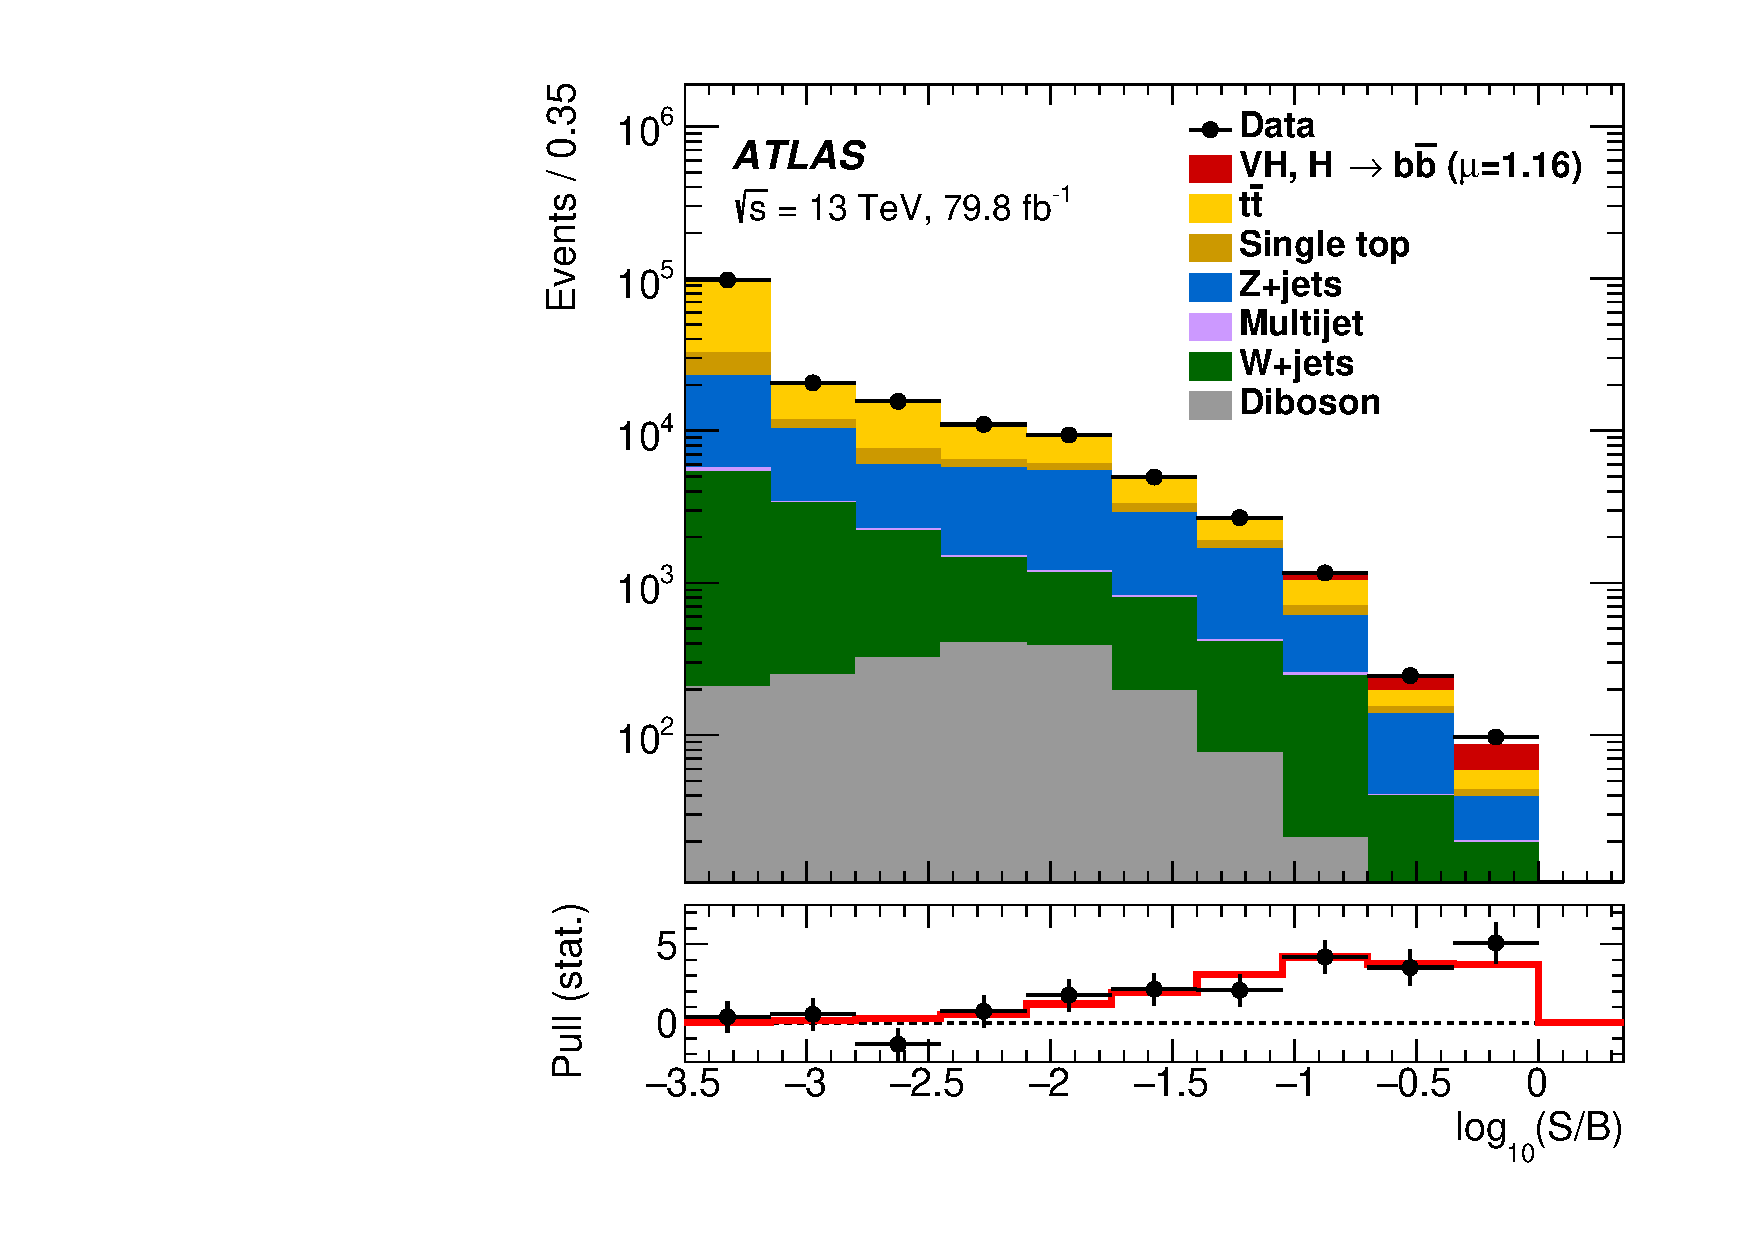
\includegraphics[width=0.85\hsize]{chapters/figures/ATLAS_VH_bb.pdf} \\
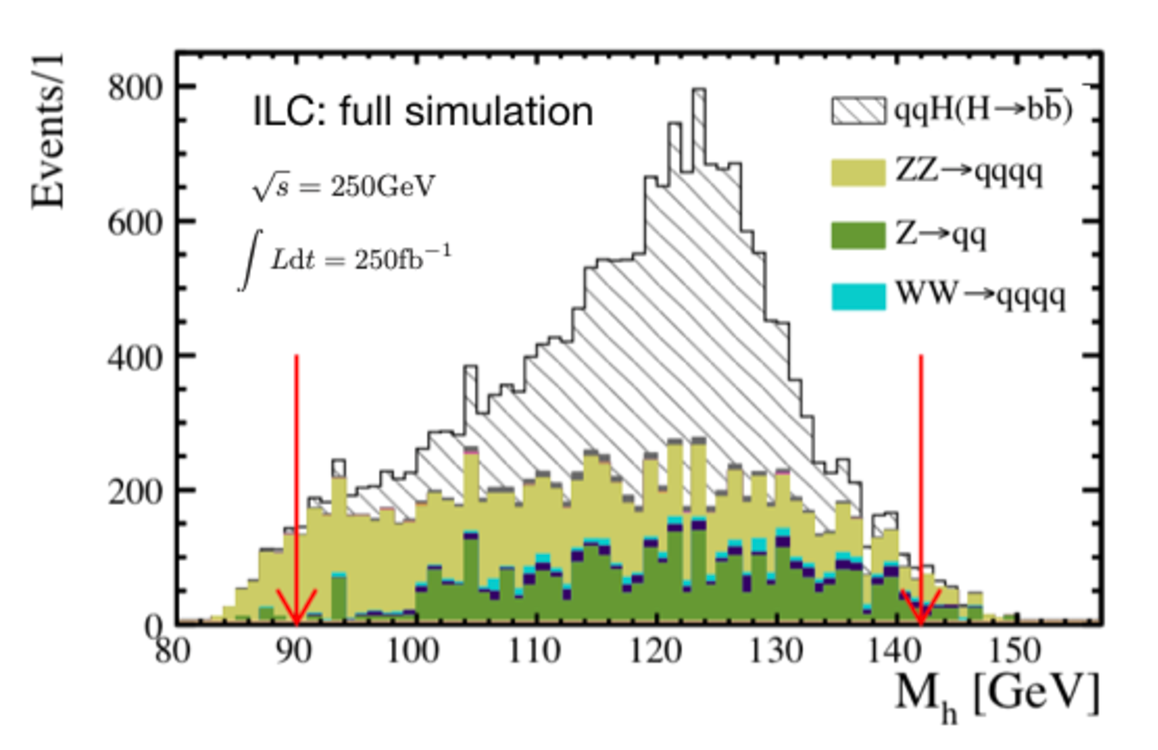
\includegraphics[width=0.85\hsize]{chapters/figures/qqH_bb250_ILC.pdf}
\end{tabular}
  \caption{Upper: signal $h\to b\bar{b}$ and background events in different categories of S/B
  measured by ATLAS~\cite{} using LHC Run 2 data; lower: signal $h\to b\bar{b}$ 
  and background events in the $b\bar{b}$ mass spectrum expected from the 
  ILC full simulation~\cite{}.}
  \label{fig:LHCILCHbb}
\end{figure}